\chapter{Projeto Sistema de Controle}

% Notas:
%   Eixos x, y e z utilizados como equações. ex: $x$, $y$ e $z$.

\label{CapProjCont}

% Resumo opcional. Comentar se não usar.
%\resumodocapitulo{Resumo opcional}

\section{Modelagem}
Para o desenvolvimento de um sistema de controle é interessante inicialmente
definir o modelo deste, identificando variáveis importantes para o sistema,
como variáveis de entrada, de saída, e variáveis controladas.

O manipulador em questão será controlado por um \textit{joystick}, 
que implementa a interface entre o sistema de controle e o usuário. 
Consequentemente, define-se como variáveis de entrada os valores 
dos eixos $x$, $y$ e $z$ lidos através do \textit{joystick}.

O efetuador final do braço robótico é o que realizará de fato a
interface entre o usuário e o ambiente, deste modo, é interessante
que o usuário tenha controle sobre à localização 3D do efetuador
no espaço e sua orientação, resultando em 6 variáveis de saída desejadas.

Como há somente 3 variáveis de entrada para controle das 6 variáveis de 
interesse, optou-se por dividir o volume de trabalho do manipulador em 
planos. Ao todo, foram criados 4 planos de ação, 2 planos de translação, 
$XY$ e $XZ$, e 2 planos de rotação, $R1$ e $R2$. Os planos de translação
fazem referência ao sistema de coordenadas global, afixado à base do 
manipulador. Já os planos de rotação foram afixados à quinta junta do manipulador, 
adotando-se que o ser humano consegue interpretar mais facilmente a rotação 
de um objeto em torno do seu próprio eixo do que em termos de rotação nos 
eixos do sistema de coordenadas global, facilitando o controle do pulso do manipulador. 

Esta organização de sub-planos de trabalho foi realizada de modo a facilitar 
o entendimento pelo usuário. Para cada plano de ação, 2 das variáveis de entrada 
serão relacionadas com as variáveis pertinentes a cada plano, alternando-se entre 
os planos de ação por meio da terceira entrada do \textit{joystick}. As variáveis dos
planos de translação estão indicas no nome do próprio plano, $XY$ ou $XZ$. Para os planos
de rotação, foram utilizados como base os eixos $\hat{Y}_5$ e $\hat{Z}_5$ para o plano
$R1$ e os eixos $\hat{Y}_5$ e $\hat{X}_5$ para o plano $R2$. Uma rotação em torno do eixo 
$\hat{Y}_5$ gera a mesma rotação em torno do eixo $\hat{Z}_6$, controlando diretamente 
a rotação do punho. Já o eixo $\hat{Z}_5$ controla a guinada, e por fim, o eixo $\hat{X}_5$
se relaciona com a arfagem, finalizando as 3 movimentações possíveis para o punho.

É necessário definir também a interação entre os dados de entrada do usuário e 
as variáveis internas do robô. Pela imensa quantidade de posições e orientações possíveis, 
adotou-se que os \textit{inputs} do usuário, limitados a dois eixos, não poderiam ser diretamente relacionados
com posições, mas sim com um desejo de movimento do robô controlado. Portanto, 
os dados lidos pelo \textit{joystick} serão transformados em velocidades a serem impostas
no efetuador final, sejam estas de translação ou rotação, a depender do plano de ação.

\section{Análise Cinemática}
\label{sec:analise-cinematica}

Como informado na seção \ref{sec:jacobiana} deste documento, a jacobiana
é uma matriz que relaciona as diversas velocidades em um manipulador 
robótico, podendo ser utilizada para representar a velocidade do efetuador final
em função da velocidade de variação dos ângulos das juntas.
Para se obter então esta relação é necessário seguir as equações de propagação
de velocidades no manipulador, \ref{eq:speed1} e \ref{eq:speed2}.
Estas equações dependem das matrizes de rotação e translação entre as 
juntas, que podem ser encontradas utilizando as regras dispostas nas 
equações \ref{eq:transform} e \ref{eq:transform2}.

Utilizando os parâmetros de DH do novo modelo, dispostos na tabela \ref{tab:DH-comparacao},
e a equação \ref{eq:transform}, foram obtidas as matrizes $^{i-1}_iT$, para $i$ de 1 a 6. 
Os resultados obtidos estão dispostos nas equações de \ref{eq:t01} a \ref{eq:t56}.
Para facilitar o entendimento, as funções trigonométricas seno e cosseno serão abreviadas pelas
letras $s$ e $c$, respectivamente.

\begin{multicols}{2}
    \noindent
    \begin{equation}
        \label{eq:t01}
        ^0_1T = \begin{bmatrix}
                    c\theta_1 & -s\theta_1 & 0 & 0 \\
                    s\theta_1 & c\theta_1 & 0 & 0 \\
                    0 & 0 & 1 & d_1 \\
                    0 & 0 & 0 & 1 \\
                \end{bmatrix}
    \end{equation}
    \begin{equation}
        ^1_2T = \begin{bmatrix}
                    c\theta_2 & -s\theta_2 & 0 & a_1 \\
                    0 & 0 & -1 & 0 \\
                    s\theta_2 & c\theta_2 & 0 & 0 \\
                    0 & 0 & 0 & 1 \\
                \end{bmatrix}
    \end{equation}
\end{multicols}

\begin{multicols}{2}
    \noindent
    \begin{equation}
        ^2_3T = \begin{bmatrix}
                    c\theta_3 & -s\theta_3 & 0 & a_2 \\
                    s\theta_3 & c\theta_3 & 0 & 0 \\
                    0 & 0 & 1 & 0 \\
                    0 & 0 & 0 & 1 \\
                \end{bmatrix}
    \end{equation}
    \begin{equation}
        ^3_4T = \begin{bmatrix}
                    c\theta_4 & -s\theta_4 & 0 & a_3 \\
                    s\theta_4 & c\theta_4 & 0 & 0 \\
                    0 & 0 & 1 & 0 \\
                    0 & 0 & 0 & 1 \\
                \end{bmatrix}
    \end{equation}
\end{multicols}

\begin{multicols}{2}
    \noindent
    \begin{equation}
        \label{eq:t45}
        ^4_5T = \begin{bmatrix}
                    s\theta_5' & c\theta_5' & 0 & a_4 \\
                    0 & 0 & -1 & 0 \\
                    -c\theta_5' & s\theta_5' & 0 & 0 \\
                    0 & 0 & 0 & 1 \\        
                \end{bmatrix}
    \end{equation}
    \begin{equation}
        \label{eq:t56}
        ^5_6T = \begin{bmatrix}
                    c\theta_6 & -s\theta_6 & 0 & 0 \\
                    0 & 0 & 1 & d_6 \\
                    -s\theta_6 & -c\theta_6 & 0 & 0 \\
                    0 & 0 & 0 & 1 \\
                \end{bmatrix}
    \end{equation}
\end{multicols}

Nota-se que para a transformação da equação \ref{eq:t45} utilizou-se a nova variável
$\theta_5'$, de acordo com a equação \ref{eq:junta5-offset}.

A transformação de um vetor expresso no sistema da última junta do punho para coordenadas
globais, ou seja, para o sistema de coordenadas da base, foi obtida através 
da multiplicação de todas as transformações, de maneira consecutiva, como indicado na
equação \ref{eq:t06}.
Esta transformação é importante para referenciar as velocidades
da ponta do manipulador para o sistema global, de mais fácil visualização e entendimento
por parte de usuários.

\begin{equation}
    \label{eq:t06}
    ^0_6T = ^B_6T = ^0_1T*^1_2T*^2_3T*^3_4T*^4_5T*^5_6T
\end{equation}

Aplicando-se então as equações \ref{eq:speed1} e \ref{eq:speed2}, e utilizando para a 
base vetores nulos de velocidades, isto é, $^0\omega_0 = \, ^0v_0 = \left[0 \; 0 \; 0 \right]^T$,
foram obtidas as velocidades lineares e angulares de todas as juntas, expressas nos seus devidos 
sistemas de coordenadas. As velocidades de interesse a serem controladas pelo usuário, ou seja,
as velocidades do final do manipulador, $\omega_6$ e $v_6$, foram remetidas ao sistema de 
coordenadas da base pré-multiplicando os vetores $^6\omega_6$ e $^6v_6$ pela matrix $^0_6Rot$,
que compõe parte da matriz $^0_6T$, previamente calculada.
Os resultados obtidos para esses dois vetores de velocidade estão dispostos nas equações 
\ref{eq:0w6} e \ref{eq:0v6}.

\begin{equation}
    \label{eq:0w6}
\begin{gathered}
    ^0\omega_6 = \begin{bmatrix}
        s\theta_1(\dot{\theta}_2 + \dot{\theta}_3 + \dot{\theta}_4) + c\theta_1s(\theta_2+\theta_3+\theta_4)\dot{\theta}_5 + \\
        + [c\theta_1c\theta_5'c(\theta_2+\theta_3+\theta_4) +s\theta_1s\theta_5']\dot{\theta}_6\\
        \\
        -c\theta_1(\dot{\theta}_2+\dot{\theta}_3+\dot{\theta}_4) + s\theta_1s(\theta_2+\theta_3+\theta_4)\dot{\theta}_5 + \\
        +[s\theta_1c\theta_5'c(\theta_2+\theta_3+\theta_4) -c\theta_1s\theta_5']\dot{\theta}_6 \\
        \\
        \dot{\theta}_1 -c(\theta_2+\theta_3+\theta_4)\dot{\theta}_5 + \\
        +c\theta_5's(\theta_2+\theta_3+\theta_4)\dot{\theta}_6 \\   
    \end{bmatrix}
\end{gathered}
\end{equation}

\begin{equation}
    \label{eq:0v6}
\begin{gathered}
    ^0v_6 = 
    \begin{bmatrix}
        % First line
        \{c\theta_1s\theta_5'd_6 - s\theta_1[a_1 + c\theta_2a_2 + c(\theta_2 + \theta_3)a_3 + c(\theta_2+\theta_3+\theta_4)(a_4 + c\theta_5'd_6)]\}.\dot{\theta}_1 - \\
        - c\theta_1[s\theta_2a_2 + s(\theta_2 + \theta_3)a_3 + s(\theta_2+\theta_3+\theta_4)(a_4 + c\theta_5'd_6)].\dot{\theta}_2 - \\
        - c\theta_1[s(\theta_2+\theta_3)a_3 + s(\theta_2+\theta_3+\theta_4)(a_4 + c\theta_5'd_6)].\dot{\theta}_3 - \\
        - c\theta_1s(\theta_2+\theta_3+\theta_4)(a_4 + c\theta_5'd_6).\dot{\theta}_4 + \\
        + [c\theta_1s\theta_5'c(\theta_2+\theta_3+\theta_4) - s\theta_1c\theta_5']d_6.\dot{\theta}_5 \\
        \\

        % Second line
        \{s\theta_1s\theta_5'd_6 + c\theta_1[a_1 + c\theta_2a_2 + c(\theta_2+\theta_3)a_3 + c(\theta_2 + \theta_3 + \theta_4)(a_4 + c\theta_5'd_6)]\}.\dot{\theta}_1 - \\
        -s\theta_1[s\theta_2a_2 + s(\theta_2+\theta_3)a_3 + s(\theta_2+\theta_3+\theta_4)(a_4 + c\theta_5'd_6)].\dot{\theta}_2 - \\
        -s\theta_1[s(\theta_2+\theta_3)a_3 + s(\theta_2+\theta_3+\theta_4)(a_4 + c\theta_5'd_6)].\dot{\theta}_3 - \\
        -s\theta_1s(\theta_2+\theta_3+\theta_4)(a_4 + c\theta_5'd_6).\dot{\theta}_4 + \\
        +[s\theta_1s\theta_5'c(\theta_2+\theta_3+\theta_4) + c\theta_1c\theta_5']d_6.\dot{\theta}_5\\
        \\

        % Third line
        [c\theta_2a_2 + c(\theta_2+\theta_3)a_3 + c(\theta_2+\theta_3+\theta_4)(a_4 + c\theta_5'd_6)].\dot{\theta}_2 + \\
        +[c(\theta_2+\theta_3)a_3 + c(\theta_2+\theta_3+\theta_4)(a_4+c\theta_5'd_6)].\dot{\theta}_3 + \\
        +c(\theta_2+\theta_3+\theta_4)(a_4+c\theta_5'd_6).\dot{\theta}_4 + \\
        +s\theta_5's(\theta_2+\theta_3+\theta_4)d_6.\dot{\theta}_5\\
    \end{bmatrix}
\end{gathered}
\end{equation}

Analisando a equação \ref{eq:mjacobiana} e sabendo que o vetor de velocidade das juntas
é um vetor coluna 6x1, $\dot{\Theta} = [\dot{\theta}_1 \; \dot{\theta}_2 \; \dot{\theta}_3 \; \dot{\theta}_4 \; \dot{\theta}_5 \; \dot{\theta}_6]^T$,
é possível escrever um vetor de velocidades do efetuador final como a junção dos vetores de velocidade linear
e angular, para obter uma matriz jacobiana quadrada, passível de ser invertida para que as velocidades das juntas
sejam representadas em função da velocidade desejada do manipulador final. Estas relações estão dispostas nas equações 
\ref{eq:jac1} e \ref{eq:jac2}.

\begin{multicols}{2}
    \noindent
    \begin{equation}
        \label{eq:jac1}
        ^0\nu = \begin{bmatrix}
                    ^0v_6 \\
                    ^0\omega_6
                \end{bmatrix}
              = \,^0\!J(\Theta)\dot{\Theta}
    \end{equation}
    \noindent
    \begin{equation}
        \label{eq:jac2}
        \dot{\Theta} = \,^0\!J^{-1}(\Theta)^0\nu = \,^0\!J^{-1}(\Theta)\begin{bmatrix}
                                                                            ^0v_6 \\
                                                                            ^0\omega_6
                                                                        \end{bmatrix}
    \end{equation}
\end{multicols}

Os termos da jacobiana podem ser obtidos através de análise das equações \ref{eq:0w6} e \ref{eq:0v6},
sendo os termos que multiplicam as derivadas dos ângulos das juntas.

Buscando-se evitar gasto excessivo de processamento na inversão desta matriz jacobiana 6x6 para cada
novo valor do vetor $\Theta$, foi realizada uma inversão simbólica da matriz, isto é, mantendo os 
valores de $\theta_1$ a $\theta_6$ como variáveis. Para inverter a matriz jacobiana foi utilizado o 
método de inversão por matriz adjunta. A equação base que rege este método está disposta em \ref{eq:inv_adjunta}.

\begin{equation}
    \label{eq:inv_adjunta}
    J^{-1}  = \frac{1}{|J|}.adj(J)
\end{equation}

Nota-se pela equação \ref{eq:inv_adjunta} que para a inversão são necessários o determinante da matriz,
identificado por $|J|$, e sua matriz adjunta. O determinante da matriz foi calculado e o resultado obtido
está definido na equação \ref{eq:det}.

\begin{equation}
    \label{eq:det}
    |J| = -c\theta_5's\theta_3a_2a_3[a_1+c\theta_2a_2+c(\theta_2+\theta_3)a_4+c(\theta_2+\theta_3+\theta_4)(a_4+2c\theta_5'd_6)]  
\end{equation}

A matriz adjunta foi então calculada a partir dos cofatores da matriz, finalizando o 
processo de inversão. 
A matriz resultante obtida foi comparada com a matriz invertida a partir dos \textit{softwares}
\textit{MATLAB} e \textit{Maple}, próprios para cálculos algébricos, verificado-se que o 
resultado obtido a partir dos cálculos manuais estava correto.

Foi escrita então uma rotina na linguagem ``c++'' que realiza a inversão da 
matriz, calculando os cofatores e determinante a partir de seus termos simbólicos. 
Visando reduzir a quantidade de cálculos a serem realizados pelo controlador, os termos da 
matriz jacobiana inversa foram reagrupados, favorecendo o reúso de variáveis.
Para verificar a rotina criada, foi escrito um \textit{script} em \textit{python}
que realizava as equações \ref{eq:jac1} e \ref{eq:jac2} em sequência, para uma 
determinada configuração de ângulos e suas velocidades, obtendo uma velocidade para 
a última junta e então realizando o processo inverso pelo uso da rotina criada, esperando-se 
obter os mesmos valores iniciais.

\section{Tratamento das variáveis de entrada}
As variáveis de entrada do sistema serão dois valores de ângulos impostos pelo
usuário ao \textit{joystick}. Para transformar estes dados em uma indicação de 
velocidade, foi necessário inicialmente realizar uma calibração dos valores lidos.
Para realizar a calibração, criou-se uma rotina que no início do sistema 
realiza uma quantidade fixa de medidas destes valores, e define um valor médio para
cada eixo, com base na média destas leituras. Para valores próximos a este valor médio,
assume-se ausência de movimento.

Para transformar os dados de leitura do \textit{joystick} em um vetor indicando
a velocidade desejada no plano de atuação do sistema, foi necessário transformar
a área efetiva de movimentação conjunta dos potenciômetros do \textit{joystick},
inicialmente um quadrado, em um círculo, com módulo máximo igual a 100\%.
Este mapeamento para uma nova área efetiva é necessário para 
garantir que todas as posições do \textit{joystick} estarão sujeitas às mesmas 
limitações de módulo, o que não é verdade para uma área em formato quadrado.

Para realizar esta transformação, é calculado o ângulo em que o \textit{joystick}
se encontra através dos valores dos eixos $x$ e $y$, é então calculado o módulo máximo 
passível de ser obtido com esse ângulo. Os novos valores de $x$ e $y$ são posteriormente
definidos com base na relação entre o módulo real do sensor e o módulo máximo, e no 
ângulo observado.

\section{Motores de passo}

Para o controle da velocidade dos motores de passo utilizou-se como base a equação
\ref{eq:stepper2}. Buscando-se definir rampas de aceleração para o acionamento
desses motores e consequentemente maior suavidade no movimento, foi formulada a equação 
\ref{eq:stepper3}.

\begin{equation}
    \label{eq:stepper3}
    \dot{\omega} = \frac{\omega_{i+1}-\omega_i}{k_{i+1}t_0}
\end{equation}

Substituindo a equação \ref{eq:stepper2} para a variável $\omega_{i+1}$
obtém-se a equação de segundo grau \ref{eq:stepper4}, que relaciona o novo 
contador $k_{i+1}$ e a velocidade atual $\omega_i$.

\begin{equation}
    \label{eq:stepper4}
    (k_{i+1}t_0)^2\dot{\omega} = \alpha_s - \omega_ik_{i+1}t_0
\end{equation}

Pela fórmula de Bhaskara, pode-se expressar o novo valor do contador completamente
em função da velocidade atual, para uma aceleração $\dot{\omega}$ definida. Esta 
solução pode ser vista na equação \ref{eq:stepper5}. A solução com valor negativo
para o resultado da raiz quadrada foi ignorada, por resultar sempre em um valor negativo,
impossível de ser atribuído a um contador.

\begin{equation}
    \label{eq:stepper5}
    k_{i+1} = \frac{-\omega_i + \sqrt{\omega_i^2+4\dot{\omega}\alpha_s}}{2t_0\dot{\omega}}
\end{equation}

Como informado na seção do controlador empregado, e seguindo a tabela \ref{tab:Pinout}, os 
pinos que geram os passos destes motores estão conectados a pinos no controlador capazes de 
gerar ondas na saída através de contadores. Dessa maneira, ao se definir uma nova 
velocidade para este tipo de motor, atribuí-se um novo valor para o registrador utilizado 
como comparador na geração destas ondas, seguindo a equação \ref{eq:stepper5}, quando for
detectado uma combinação entre um contador do sistema e o valor configurado, uma sub-rotina
será chamada que alterará o valor do pino definido como saída.

Como os motores de passo não possuem sensores para conhecimento da posição absoluta,
foi definido um momento de calibração para estes motores. No momento de início do programa, 
todos os motores de passo serão acionados com uma certa velocidade até atingir algum sensor 
fim-de-curso, que permite assumir uma posição inicial bem definida para as juntas onde estes
atuadores são empregados. A posição inicial assumida para os três motores de passo do sistema
foram: 

\begin{itemize}
    \item Junta 1: $\pi/2$ rad;
    \item Junta 5: $-\pi/2$ rad;
    \item Junta 6: $0$ rad.
\end{itemize}

\section{Motores DC}

Para controle dos motores DC, foi utilizada uma interrupção periódica no sistema do controlador,
semelhante aos pulsos gerados nos motores de passo, para atualizar o valor de tensão enviada
ao motor. 

Inicialmente, adotou-se uma relação direta entre o ciclo de trabalho de sinais PWM enviados 
ao \textit{driver} do motor e a velocidade de saída, baseando-se no regime permanente 
que seria obtido seguindo a equação \ref{eq:motordc-tf}. Desse modo, para cada motor
DC do sistema, quando a interrupção é gerada, o valor de PWM enviado ao motor é atualizado
multiplicando a velocidade desejada por uma constante, definida empiricamente para cada motor.

Também foi necessário se atentar para os funcionamentos não-lineares apresentados pelos motores
DC, especialmente os valores da zona morta dos motores. Desse modo, caso o valor obtido para
o \textit{duty cycle} esteja abaixo de um certo limiar, o valor será atualizado para este limiar.

Para aprimorar o controle dos motores DC, a função chamada quando da ocorrência da 
interrupção programada no sistema pode ser preparada para operar como parte de um sistema
de controle digital, após devidamente identificados os parâmetros de funcionamento dos
motores.

\section{Fluxograma de operação}

O código principal do sistema de controle foi dividido em sub-rotinas bem definidas, que
em conjunto promovem a movimentação e/ou simulação do sistema robótico. Uma ilustração das
etapas do sistema de controle pode ser vista na figura \ref{fig:fluxograma}.

\begin{figure}[h]
    \caption{Fluxograma do sistema de controle.}

    \begin{centering}
        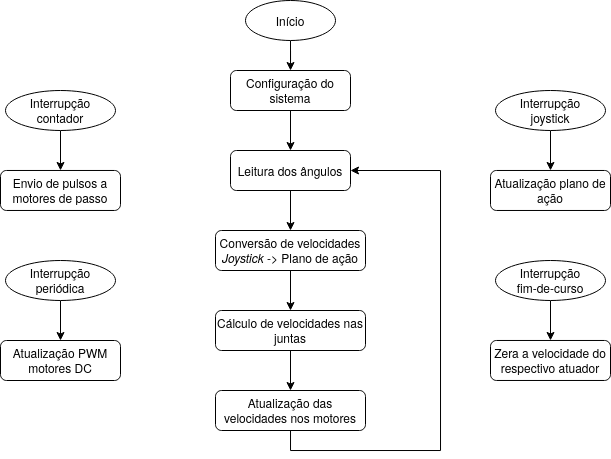
\includegraphics[width=0.7\columnwidth]{images/controle/fluxo.png} 
    \par\end{centering}

    \label{fig:fluxograma}
\end{figure}

Os símbolos ovais indicam as fontes de chamadas a sub-rotinas do código, sendo a fonte 
de início principal, a alimentação do sistema. Assim que é energizado, o sistema é iniciado, sendo
então configurado. Para a definição e configuração do sistema manipulador, foram criadas 
bibliotecas que permitem descrever um manipulador robótico e os atuadores empregados de maneira 
intuitiva e genérica, facilitando o entendimento e modificação do código, através da aplicação de 
técnicas de programação orientada a objetos. Durante a configuração os diversos equipamentos do sistema
serão calibrados e preparados para amplo funcionamento.

As outras fontes de chamadas a sub-rotinas são as interrupções, tanto aquelas geradas pelos contadores
dos motores de passo, quantos as interrupções geradas periodicamente para controle dos motores DC e 
as interrupções geradas por sensores do sistema, como fim de curso ou pelo terceiro eixo do \textit{joystick}. 
Estas interrupções são iniciadas e preparadas no momento de configuração do sistema.

Após a configuração geral do sistema, o laço de repetição principal do sistema é iniciado. 
A primeira tarefa a ser realizada é a leitura de todos os ângulos do sistema, para conhecimento
do estado geral do robô. Após a leitura dos ângulos, são lidos os dados de entrada provindos do 
usuário, e estes valores são então convertidos para as variáveis pertinentes a um dos 4 planos de
ação definidos para o sistema.
Caso o plano de ação 
atual seja um plano de rotação, assume-se que as velocidades indicadas estão representadas no
plano de coordenadas da junta 5, portanto, são transportadas para o eixo de coordenadas da base
por uma pré-multiplicação pela matriz $^0_5Rot$.

Na etapa de cálculo da velocidade nas juntas o vetor de velocidades gerado na etapa anterior será 
transformado para velocidades a serem impressas nos atuadores do sistema, através de chamada
à sub-rotina que implementa a matriz jacobiana inversa do sistema.

A etapa de atualização das velocidades nos motores realizará de fato chamadas à métodos
dos objetos que representam os atuadores do sistema para configurar a estes uma nova referência 
para sua velocidade de rotação. A manutenção desta velocidade será função das sub-rotinas 
chamadas pelas interrupções.

\section{Simulação}

Para verificar o correto funcionamento do sistema de controle, independente dos circuitos de
sensoriamento e acionamento, foi implementada uma função que simula os ângulos de leitura do sistema. 
Para utilização desta função é suficiente alterar no código fonte do programa uma diretiva
definitada como ``\textit{SIMULATION}'' para o valor 1.
Esta função atualiza os valores de ângulos do sistema com base na velocidade a ser imposta nos atuadores
e a quantidade de tempo decorrente durante a execução do laço de repetição principal. 

Com o objetivo de informar estes ângulos a um ambiente externo, foi criada outra rotina que envia os dados 
dos ângulos, lidos e/ou simulados, para algum dispositivo conectado através de uma conexão serial.

Para obtenção dos ângulos e simulação do manipulador de forma visual, o módulo criado para a 
realização das equações de Newton-Euler foi modificado para permitir o desenho do manipulador
na tela de um computador. Foi então codificada uma interface que realiza a comunicação entre o 
sistema na placa controladora Arduino e o módulo em \textit{python} modificado.

Com a possibilidade de simulação e função de comunicação com módulo de simulação, o 
novo fluxograma de controle pode ser visto na figura \ref{fig:fluxograma2}. 

\begin{figure}[h]
    \caption{Fluxograma do sistema de controle com simulação.}

    \begin{centering}
        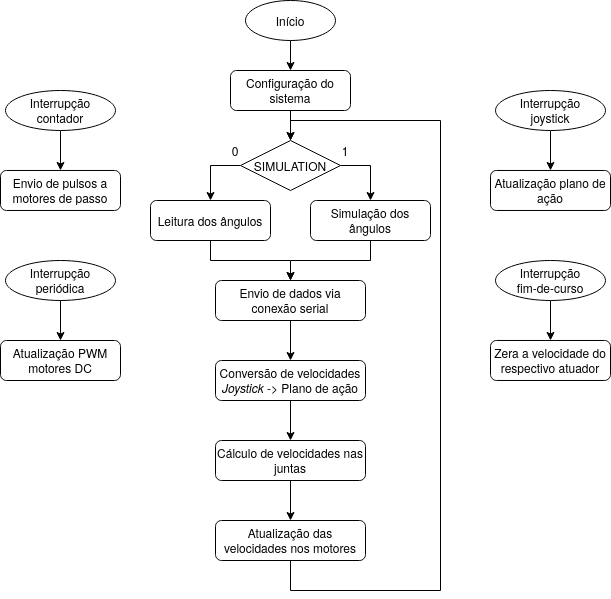
\includegraphics[width=0.7\columnwidth]{images/controle/fluxo2.png} 
    \par\end{centering}

    \label{fig:fluxograma2}
\end{figure}

O ambiente de simulação gerado realiza a animação do manipulador em tempo real, com os dados advindos
do Arduino. Este se mostrou eficiente na reprodução dos movimentos do robô quando não
foi possível utilizar a estrutura mecânica real deste para testes e validação dos circuitos. 
O módulo responsável pela animação foi projetado e codificado de maneira responsiva a mudanças, 
modificando automaticamente as escalas dos três eixos para otimizar o espaço de visualização do robô.

Um exemplo de simulação utilizando o ambiente pode ser visto em \ref{fig:exemplo}, onde foi montado 
um robô genérico com 6 graus de liberdade. As linhas em preto indicam uma conexão direta entre os sistemas 
de referência, e não necessariamente os elos do manipulador.

\begin{figure}[h]
    \caption{Exemplo de robô criado no \textit{software} simulador.}

    \begin{centering}
        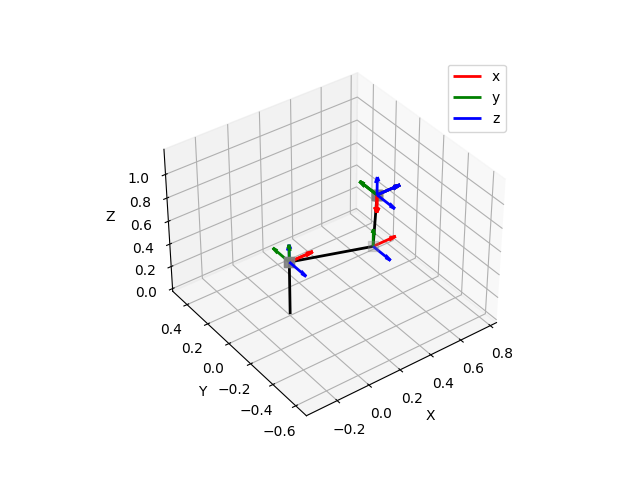
\includegraphics[width=0.8\columnwidth]{images/controle/simu-puma.png} 
    \par\end{centering}

    \label{fig:exemplo}
\end{figure}